\chapter{Instruction Level Parallelism}

\textsc{Definição} o grau no qual instruções de um mesmo programa podem ser avaliadas em paralelo, ou seja, \textbf{a medida de sobreposição potencial entre as instruções}.

\textbf{Note que:} O pipelining é uma das técnicas que explora ILP e é geralmente a base para as demais otimizações propostas.

Um programa pode ser definido como a composição de dois tipos de instruçoes:
\begin{itemize}
  \item \textbf{Atribuições}, da forma $A = B + C$;

  \item \textbf{Branches}, resultando em desvios no fluxo de execução das instruções (condicionais e laços).
\end{itemize}

O código executado entre dois \textit{branches}, i.e. um bloco básico ou \textit{branch path}, é sequencial. Logo, ele é o candidato óbvio para a exploração de paralelismo. No entanto, estudos mostram que tipicamente, o tamanho deste bloco é pequeno, indo de 3 a 0 instruções. Além disso, depêndencias existentes dentro deste bloco acabam por limitar o paralelismo.

Dessa forma, uma técnica efetiva de exploração da ILP deve ser capaz de explorar o paralelismo entre blocos distintos. Os candidatos mais fáceis para tal são as interações de um \textit{loop} - o \textit{loop level parallelism}.

% TODO: por o código
\underline{Exemplo:} aqui, cada iteração do \textit{loop} pode ser executada simultaneamente, apesar de haver a dependência de dados no interior de cada iteração.

\subsubsection{Tarefas do Compilador}
Para manter um pipeline cheio, o paralelismo entre as instruções deve ser explorado de maneira a obter sequências de instruções independentes que possam ser sobrepostas no pipeline. Duas sequências dependentes devem ser separadas por uma distâncias que seja igual à latência do pipeline para a primeira instrução, em ciclos de clock.

A habilidade do compilador de separar instruções está limitada por dois fatores:
\begin{itemize}
  \item A quantidade de ILP presente no programa

  \item As latências das unidades funcionais do pipeline
\end{itemize}

\subsubsection{Quando e Como Explorar o ILP}
Existem diversas técnicas para explorar ILP, onde a maioria necessita que se saiba quando e como a ordem das instruções de um programa pode ser alterada sem que sejam produzidos resultados incorretos.

Deve-se então saber a dependência entre as instruções para se determinar uma maneira de reordená-las sem que as dependências sejam violadas.





\section{Depêndencias}
O grau de dependência entre as instruções determina quanto paralelismo existe em um programa e como o mesmo pode ser explorado. \textbf{Duas instruções serão paralelas quando podem ser executadas simultaneamente em um pipeline, sem a necesidade de atrasos.} Se duas instruções não são paralelas, então elas \textbf{são dependentes} e logo não podem ser reordenadas.

Dependências são propriedades de programas e a presença delas indica o potencial para atrasos no pipeline. Porém, qual atraso e seu impacto é uma propriedade do pipeline.




\subsection{Dependências de Dados}
\textsc{Definição} quando uma instrução depende do resultado de uma instrução específica ou do resultado encadeado de instruções, então temos uma dependência de dados. Também chamada de dependência real.

\begin{figure}[ht]
  \centering
  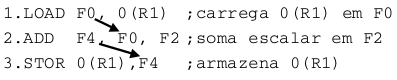
\includegraphics[width=0.6\textwidth]{data-dependency}
  \caption{Aqui, temos uma dependência encadeada: a instrução 3 depende da 2, que depende da 1}
  \label{fig:data-dependency}
\end{figure}

A existência de dependência de dados implica na existência de uma cadeia de \textit{hazards} RAW entre as instruções. Caso as instruções dependentes de dados sejam escalonadas simultaneamente, o pipeline será atrasado.

Uma dependência de dados possui as seguintes características:
\begin{itemize}
  \item Indica a possibilidade de um atraso no pipeline;
  \item Determina em que ordem as operações devem ser executadas;
  \item Determina um limite superior na quantidade de paralelismo que pode ser explorada
\end{itemize}

Pelo fato delas limitarem a ILP, elas devem ser tratadas. Temos duas maneiras:
\begin{itemize}
  \item \textbf{Manter a dependência}, evitando o atraso, o que pode ser feito pelo pipeline ou pelo compilador;

  \item \textbf{Rearrumar o o código} de maneira a eliminar a dependência, feito apenas pelo compilador
\end{itemize}

Um valor de dado pode fluir entre instruções através de registradores ou posições de memória. \textbf{Por um registrador, a detecção de dependência é mais simples, pois os nomes são fixos}. As dependências que ocorrem através de posições de memória possuem um tratamento mais difícil.

\underline{Exemplo:} 100(R2) e 20(R4) podem endereçar a mesma posição de memória, mas é dificil o compilador saber disso. Logo, ele toma o caminho mais conservador que é manter a dependência.





\subsection{Dependências de Nomes}
\textsc{Definição} quando não há valor transferido entre instruções, mas ambas usam o mesmo nome (de registrador ou posição de memória) e pelos menos uma delas altera o valor deste nome, temos uma dependência de nome. Temos dois tipos:

\begin{itemize}
  \item \textbf{Anti-Dependência:} ocorre quando uma instrução lê o valor de um nome e uma outra instrução quer escrever neste mesmo nome. Ou seja, quando \textbf{temos um WAR}. \underline{Exemplo:}

  \begin{center}
    \texttt{ADD R1, R1, R3}\\
    \texttt{LOAD R3, 0(R4)}\\
  \end{center}

  \item \textbf{Dependência de Saída:} ocorre quando duas instruções querem escrever no mesmo nome. Ou seja, quando \textbf{temos um WAW}.
  \underline{Exemplo:}

  \begin{center}
    \texttt{LOAD R1, 0(R2)}\\
    \texttt{ADD R1, R1, 10}\\
  \end{center}
\end{itemize}

Como não há valor sendo transmitido entre instruções, as dependências de nomes são mais fáceis de serem eliminadas se o nome utilizado for alterado, de maneira a remover o conflito. Chamamos isso \textbf{register renaming}. Esta renomeação pode ser feita tanto por \textit{hardware} como por compilador.






\subsection{Dependências de Controle}
\textsc{Definição} quando o ordenamento de uma instrução está atrelado a um \textit{branch}, temos uma dependência de controle.

Toda a instrução, exceto as pertencentes ao primeiro bloco básico, estão atreladas a algum conjunto de \textit{branches} e logo é dependente de controle destes. No caso geral, as dependências de controle devem ser preservadas.

\underline{Exemplo:} vemos abaixo que \texttt{s1} é dependente de \texttt{p1}. Já \texttt{s2} é dependente de \texttt{p2}, mas não de \texttt{p1}\\

\texttt{if (p1) \{ \\  s1\\\}\\if(p2)\{\\  s2\\\}}

Essas dependências geram duas restrições:
\begin{itemize}
  \item Uma instrução que é dependente de controle de um branch não pode ser movida para antes deste branch;

  \item Uma instrução que não é dependente de controle de um branch não pode ser movida para depois do branch, pois caso fosse, sua execução seria então controlada por ele.
\end{itemize}

Em um pipeline básico, as dependências de controle são preservadas por dois motivos:
\begin{itemize}
  \item As instruções são executadas em ordem;

  \item Uma instrução que é dependente de um branch não é executada até que a direção do branch seja conhecida, devido aos hazards de controle.
\end{itemize}

As propriedades a seguir são preservadas pela dependência de controle afim de garantir a correção do programa.



\subsubsection{Comportamento em Face a Exceções}
O reordenamento da execução de das instruções não deve permitir o surgimento de exceções no programa. Por isso, uma postura conservadora é adotada e o reordenamento não é feito, mesmo que não haja dependência de dados.

\begin{figure}[ht]
  \centering
  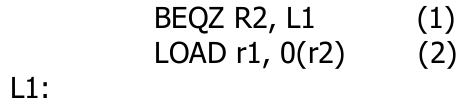
\includegraphics[width=0.6\textwidth]{except-behavior}
  \caption{Se ignoramos a dependência de controle entre 1 e 2, se a instrução 2 é executada antes do branch, podemos levar a um estado de erro, o que não ocorreria se o branch fosse tomado}
  \label{fig:except-behavior}
\end{figure}



\subsubsection{Fluxo de Dados}
\textsc{Definição} o fluxo real de dados entre as instruções que os produzem e as que os consomem.

O branches fazem com que o fluxo de dados seja dinâmico, permitindo que o dado utilizado em determinada instrução possa vir de vários pontos. Logo, o reordenamento não pode afetar este fluxo.

\begin{figure}[ht]
  \centering
  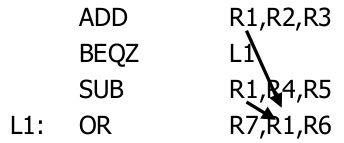
\includegraphics[width=0.6\textwidth]{data-flux}
  \caption{O valor de R1 em 4 vem de 1 se o desvio for tomado e de 3 se não for}
  \label{fig:data-flux}
\end{figure}




\section{Paralelismo a Nível de \textit{Loop}}
A maneira mais simples de se detectar paralelismo é no interior de \textit{loops}. A análise de paralelismo neste nível consiste em se determinar se acesso a dados em iterações posteriores são dependentes de valores de iteração anteriores, i.e., se $i$ depende de $i-1$. Geralmente, esta análise é feita no código fonte, pois a tradução pra a linguagem de máquina cria dependências no registrador de incremento de índice. As Figuras \ref{fig:loop-pal-1}, \ref{fig:loop-pal-2} e \ref{fig:loop-pal-3} refletem bem isso.

\begin{figure*}
  \begin{subfigure}{.45\textwidth}
    \centering
    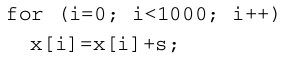
\includegraphics[width=0.9\textwidth]{loop-pal-1}
    \caption{Aqui a dependência ocorre entre os dois usos de \texttt{x{[i]}}, sendo interna a cada iteração. Entre \textit{loops} não há dependencia e eles são paralelos}
    \label{fig:loop-pal-1}
  \end{subfigure}
  ~
  \begin{subfigure}{.45\textwidth}
    \centering
    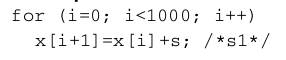
\includegraphics[width=0.9\textwidth]{loop-pal-2}
    \caption{Aqui, \texttt{x{[i+1]}} e \texttt{x{[i]}} dependem, criando dependência entre os laços, obrigando-os a serem executados em ordem. Chamamos esse tipo de \textbf{loop-carried dependencie}}
    \label{fig:loop-pal-2}
  \end{subfigure}
  ~
  \begin{subfigure}{\textwidth}
    \centering
    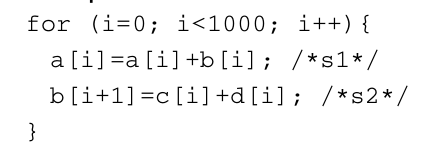
\includegraphics[width=0.5\textwidth]{loop-pal-3}
    \caption{Aqui a dependência é entre \texttt{s1} e \texttt{s2}, pelo fato de \texttt{b{[i]}} depender de \texttt{b{[i+1]}}. Mas note que \texttt{s2} não depende de \texttt{s1}}
    \label{fig:loop-pal-3}
  \end{subfigure}

  \caption{Avaliações de paralelismo a nível de \textit{loop}}
\end{figure*}

Um loop é paralelo se puder ser escrito de maneira que não haja dependência circular entre as dependências \textit{loop-carried}. Note no exemplo da Figura \ref{fig:loop-pal-2} que a dependência é circular, pois \texttt{s1} depende dela própria.

No exemplo da Figura \ref{fig:loop-pal-3}, não há dependência circular, pois \texttt{s2} não depende de \texttt{s1} (mas \texttt{s1} depende de \texttt{s2}). Logo, podemos reescrevê-lo afim de se tornar paralelo. A Figura \ref{fig:loop-pal-fix} mostra o conserto.

\begin{figure}[ht]
  \centering
  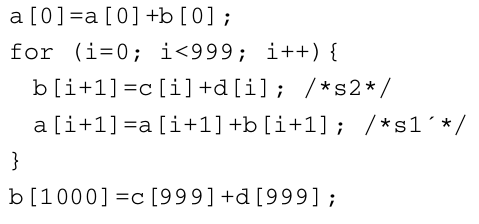
\includegraphics[width=0.6\textwidth]{loop-pal-fix}
  \caption{Agora o loop pode ser paralelo. Semelhante ao exemplo na Figura \ref{fig:loop-pal-1}}
  \label{fig:loop-pal-fix}
\end{figure}






\section{Semântica e Notações de Desvios}
Em desvios condicionais, se a condição for verdadeira, o controle é transferido para a instrução destino do branch - a \textit{branch target address} - e neste caso é dito \textbf{tomado (\textit{taken - T})}. Se a condição é falsa, a execução continua com a instrução imediatamente posterior ao \textit{branch} e o desvio é dito \textbf{não tomado (\textit{not taken - NT})}.

O desvio pode ser \textit{backwards}, indo para trás ou \textit{forward}, indo para frente.



\subsection{Previsões}
Os sinais dos desvios são geralmente preditos por esquemas de previsão de desvio e medimos sua acurácia: \textit{branch prevision accuracy}, ou BPA. O caminho predito é o \textit{predicted path} e o caminho cuja previsão diz que não será tomado é o \textit{not predicted path}.

\textsc{Definição} \textbf{Janela de execução do processador:} parte do código que está em processo de execução na CPU

Um desvio é geralmente previsto depois que entra na janela de execução. Após a previsão, o desvio fica \textbf{pendente}. Quando a condição do desvio é efetivamente avaliada, o branch é dito \textbf{resolvido}.

\textsc{Definição} \textbf{Código estático:} código na ordem de escrita pelo programador ou compilador.

\textsc{Definição} \textbf{Código dinâmico:} diferentes instâncias de instruções estáticas, que surgem durante a execução, ordenadas pelo tempo no qual foram executadas.







\section{Técnicas de Exploração}

\subsection{\textit{Loop Unrolling}}
\textsc{Definição} aumento do bloco básico entre as iterações de um \textit{loop}.

É uma das técnicas mais simples para explorar ILP e implica em um rearrumação do código, normalmente feita pelo compilador. Aplicamos tal técnica em loops independentes, ou seja, loops paralelos. As Figuras \ref{fig:loop-unrolling-1} e \ref{fig:loop-unrolling-2} explicam bem.

Apesar do \textit{loop unrolling} aumentar o tamanho do código do programa, esta transformação é bastante utilizada pois permite o uso mais eficiente do pipeline.

\begin{figure*}
  \begin{subfigure}[b]{.45\textwidth}
    \centering
    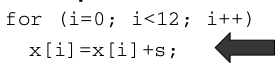
\includegraphics[width=0.9\textwidth]{loop-unrolling-1}
    \caption{Loop paralelo, com bloco básico pequeno}
    \label{fig:loop-unrolling-1}
  \end{subfigure}
  ~
  \begin{subfigure}[b]{.45\textwidth}
    \centering
    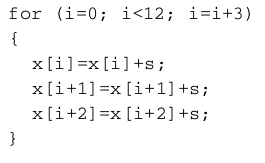
\includegraphics[width=0.9\textwidth]{loop-unrolling-2}
    \caption{Bloco básico estendido e número de iterações menor}
    \label{fig:loop-unrolling-2}
  \end{subfigure}

  \caption{Exemplo de \textit{loop unrolling}}
\end{figure*}


\subsection{Escalonamento Dinâmico}
Permite que o \textit{hardware} reordene a execução das instruções de maneira a reduzir os atrasos no pipeline. Como a reordenação é feita em tempo de execução, o escalonamento é dinâmico. Ele pode ser combinado com o escalonamento estático.

Como \textbf{vantagens}, podemos tratar situações onde as dependências não são conhecidas em tempo de compilação e permite que o código que foi compilada para um tipo de pipeline rode eficientemente em outro tipo. Como \textbf{desvantagens}, temos o aumento da complexidade de \textit{hardware}.

O pipeline básico faz a busca de instruções na ordem do programa. Neste caso, se uma instrução atrasa o pipeline - ou seja, geral um \textit{stall} - nenhuma outra instrução pode prosseguir.

\begin{figure}[ht]
  \centering
  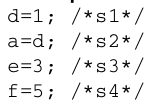
\includegraphics[width=0.4\textwidth]{dynamic-escalo-ex}
  \caption{A instrução \texttt{s2} necessita de \texttt{s1}. Porém, \texttt{s3} e \texttt{s4} são atrasadas, mesmo não dependendo de \texttt{s1} e \texttt{s2}. Podemos eliminar isto se executarmos fora de ordem}
  \label{fig:dynamic-escalo-ex}
\end{figure}

A execução fora de ordem permite que as instruções possam começar sua execução no momento em que seus operando estão disponíveis. Ela também implica que o término das instruções também será fora de ordem, o que pode gerar erros, complicando o tratamento de exceções.

A execução fora de ordem divide o estágio ID em duas partes:
\begin{itemize}
  \item \textbf{Issue:} decodifica as instruções e verifica hazards estruturais

  \item \textbf{Read Operands:} espera até que não haja hazards de dados e lê operandos.
\end{itemize}

A execução de uma instrução se inicia no instante $t$ e termina no instante $v$, onde $v > t$. Em um pipeline com escalonamento dinâmico, todas as instruções entram no estágio \textit{issue} na ordem do programa. Entretanto, no estágio \textit{read operands}, elas podem ser atrasadas ou fazerem um \textit{bypass} das outras instruções - o que é a própria execução fora de ordem.



\subsection{Scoreboarding}
Técnica que permite que as instruções sejam executadas fora de ordem, quando há recursos suficientes e independência de dados. O \textit{scoreboarding} é o elemento principal desta técnica, pois ele controla a execução das instruções e faz a detecção de \textit{hazards}.

Como várias instruções podem estar no estágio EX simultaneamente, o \textit{scoreboarding} \textbf{só é efetivo quando há múltiplas unidades funcionais}.

Toda a instrução que está ou já passou no estágio \textit{issue}, mas não foi terminada, possui um entrada no \textit{scoreboarding}. Ele mantem todas as informaçoes necessárias para detectar as dependências de dados.

O \textit{scoreboarding} determina o instante no qual a instrução pode ler os operando e iniciar a execução. Caso não seja possível, ele monitora toda mudança no \textit{hardware} para determinar quando uma instrução pode ser executada. Por isso, ele controla também quando o resultado pode ser escrito no estágio WB.

Suas etapas são:
\begin{itemize}
  \item \textbf{Issue:} se a unidade funcional destino estiver livre e nenhuma instrução ativa tiver o mesmo registrador destino, o scoreboard faz um issue da instrução. Essas garantias previnem \textit{hazards} WAW.

  \item \textbf{Read Operands:} o scoreboard verifica se os operandos estão disponíveis, ou seja, se nenhuma instrução anterior vai escrever neles. Caso estejam disponíveis, o scoreboard instrui a unidade funcional para a leitura dos mesmos e o início da execução;

  \item \textbf{Execution:} ao receber os operandos, a unidade funcional inicia a execução. Quando o resultado final estiver pronto, o scoreboard é notificado;

  \item \textbf{Write Result:} o scoreboard recebe a notificação e verifica a existência de hazards. Uma instrução $i$ é impedida de escrever seu resultado quando existe uma instrução $j$, precedente a $i$, que não leu os operandos e um dos operandos de $j$ é o resultado de $i$. Ou seja, uma instrução é impedida de escrever seu resultado quando este é o operando de uma outra instrução anterior, que ainda não leu os operandos.
\end{itemize}

A estrutura de dados do \textit{scoreboarding} possui 3 partes:
\begin{itemize}
  \item \textbf{Estado da Instrução:} indica em qual estágio cada instrução está

  \item \textbf{Estado da Unidade Funcional:} possui 9 campos para cada unidade funcional. Eles são: busy, operação, registrador destino (Fi), registradores fonte (Fj,Fk), unidades funcionais que produzem os registradores fonte (Qj,Qk) e flags indicando se os registradores fonte estão prontos (Rj,Rk);

  \item \textbf{Estado do Registrador Resultado:} indica a unidade funcional que escreverá cada registrador
\end{itemize}

O \textit{scoreboarding} apresenta algumas \textbf{deficiências}:
\begin{itemize}
  \item Necessitava de um grande número de barramentos

  \item A escolha das instruções se resumia a um mesmo bloco básico, o que não trás grande paralelismo.
\end{itemize}




\subsection{Tomasulo}
Combina o \textit{scoreboarding} com renomeação de registradores. Possui unidades chamadas \textbf{estações reservas}. Elas servem para armazenar os operando das operações que estão esperando o \textit{issue}, buscando-os logo que os mesmo estiverem disponíveis.

Quando várias escritas são feitas para o mesmo registrador, somente o último é utilizado. Note que os valores anteriores ao último não importam para instruções após a escrita do último. Quando operações são iniciadas, os registradores que contem operando pendentes são renomeados para os nomes das estações reservas, uma vez que elas contém os valores anteriores desse registrador. \textbf{Isso previne \textit{hazards} WAR e WAW}. Como pode haver mais estações reserva do que registradores reais, esta técnica \textbf{pode eliminar mais hazards do que o compilador poderia fazer}.

Cada unidade funcional possui estações reservas próprias, que controlam quando uma instrução pode ser executada naquela unidade, o que garante um controle descentralizado. Os valores dos operandos são obtidos pelas unidades funcionais através de barramentos compartilhados. Isso permite que todas as unidades possam obter o operando simultaneamente. \textit{Loads} e \textit{stores} são tratados como unidades funcionais.

As estações reservas acabam por guardar:
\begin{itemize}
  \item As instruções esperando por execução;
  \item Os operandos destas instruções já calculados ou então a fonte destes;
  \item Informações de controle da execução da instrução.
\end{itemize}

\begin{figure}[ht]
  \centering
  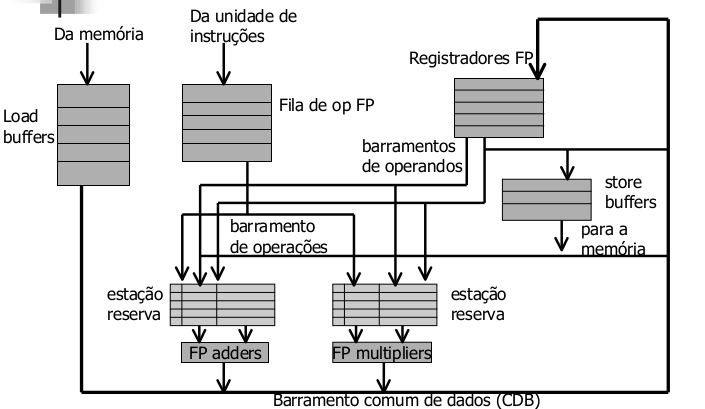
\includegraphics[width=\textwidth]{tomasulo-arch}
  \caption{Arquitetura do Tomasulo}
  \label{fig:tomasulo-arch}
\end{figure}

Temos os seguintes estágios nesta arquitetura:
\begin{itemize}
  \item \textbf{Issue:} retira uma instrução da fila de operações de ponto flutuante. Se há estação reserva livre, inicia a instrução e envia os operandos disponíveis para a estação reserva. Loads e stores podem prosseguir se houver um buffer disponível. Faz também a renomeação dos registradores

  \item \textbf{Execute:} se algum operando não estiver disponível, monitora o CDB. Quando todos os operandos estiverem disponíveis, recupera-os da estação reserva e executa a operação, se não houver hazards RAW;

  \item \textbf{Write Result:} quando o resultado estiver disponível, escreve-o no CDB e também em registradores ou estações reserva que estiverem esperando.
\end{itemize}

A estrutura de dados do Tomasulo possui 6 campos:
\begin{itemize}
  \item \textbf{$Op$:} operação a ser executada

  \item $Q_i$, $Q_j$: estações reserva que produzirão o operando fonte, onde o valor 0 indica que o operando já está disponível ou não é utilizado;

  \item \textbf{$V_i, V_j$:} valor dos operandos $i$ e $j$;

  \item \textbf{Busy/Free}
\end{itemize}

Em termo de \textbf{vantagens} o Tomasulo provê um hardware distribuido para detectar \textit{hazards} RAW e elimina os \textit{hazards} WAW e WAR, através da renomeação de registradores nas estações reservas.

Como \textbf{desvantagens}, temos um necessidade de hardware complexo, o barramento comum dos dados (CDB) pode se tornar um gargalo e não trata o problema dos desvios.






\subsection{Previsão Dinâmica de Desvios}
A frequência dos \textit{branches} torna necessária a utilização de técnicas para reduzir os atrasos potenciais causados por estes desvios, sendo as dependências de controle um grande limitador para a ILP. Nos esquemas de previsão estática de desvios, o comportamento em tempo de execução de cada desvio não é levado em conta. Toda decisão recai sobre o compilador.

A previsão dinâmica de desvios usa o hardware para analisar comportamentos
passados do branch, prevendo seu próximo resultado. A \textbf{efetividade de um esquema de previsão de branches} depende de sua acurácia e do custo de uma previsão correta e de uma previsão incorreta.

Normalmente, os previsores se baseiam em uma tabela de histórico de desvios, chamada \textit{branch history table}, ou \textbf{BHT}. Ela é uma pequena memória, indexada pela porção menos significativa do endereço da instrução de branch, que contem um bit indicando se o desvio foi recentemente tomado ou não.


\subsubsection{Previsão One-bit}
O esquema mais simples de previsão, o qual utiliza a BHT. Prevê que o branch sempre vai ser executado da maneira que foi executado na iteração anterior. Logo, o diagrama de estados segue o mostrado na Figura \ref{fig:one-bit}. Se o \textit{branch} é tomado, a busca instruções continua a partir do endereço do \textit{target} do desvio.

\begin{figure}[ht]
  \centering
  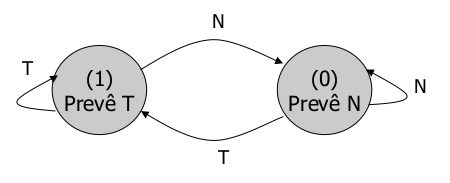
\includegraphics[width=0.75\textwidth]{one-bit}
  \caption{Autômato da Previsão One-Bit}
  \label{fig:one-bit}
\end{figure}

A previsão é uma dica sobre a direção do desvio e a carga de instruções começa a ser prevista. Se a dica estiver errada, o bit de previsão é invertido. Idealmente, deve haver um autômato por \textit{branch} estático. Possui acurácia de 77-79\% e é usado no DEC Alpha 21064, com 2K autômata.

Este esquema tem problemas com loops, onde geralmente ocorrem 2 previsões incorretas.




\subsubsection{Previsão Two-bit}
% TODO: explicar melhor cada autômato

Foi proposto para sanar a deficiênia do esquema de 1 bit, onde agora para haver a alteração de estado, a previsão deve ser incorreta por duas vezes, no mínimo. É possível haver esquemas $n$-bits, onde o de 2-bits faz parte. Um contador é incrementado quando o desvio for tomado e decrementado quando não for. Quando este for maior que $\frac{(2^n - 1)}{2}$, a previsão do desvio é T. Caso contrário, é NT.

A acurária aqui é de de 78-89\% (SPECInt89) e é utilizado no NexGen 586 (2K automata) e no Pentium (256 automata).

\begin{figure*}
  \begin{subfigure}{.5\textwidth}
    \centering
    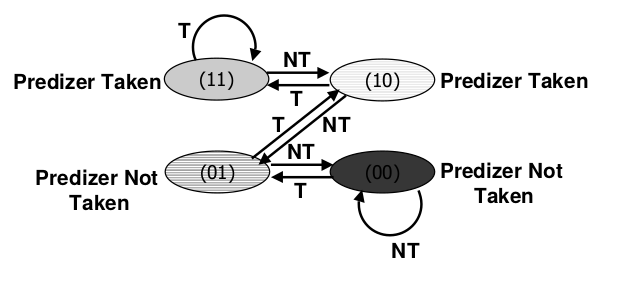
\includegraphics[width=.95\textwidth]{two-bit-sature}
    \caption{Two-Bit Saturada}
    \label{fig:two-bit-sature}
  \end{subfigure}
  ~
  \begin{subfigure}{.5\textwidth}
    \centering
    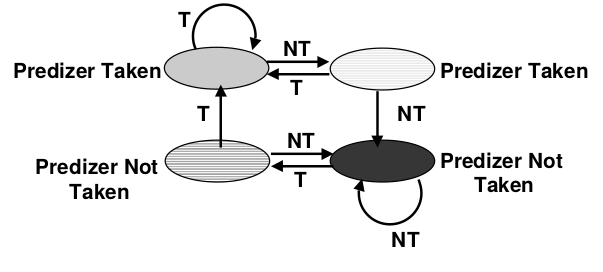
\includegraphics[width=.95\textwidth]{two-bit-patterson}
    \caption{Two-Bit Patterson}
    \label{fig:two-bit-patterson}
  \end{subfigure}
\end{figure*}




\subsubsection{Previsores Correlatos (ou de dois níveis)}
% TODO: melhorar a descrição de funcionamento do funcionamento

Muitas vezes, o comportamento de um branch está relacionado com o comportamento de outro branch. Por isso, os previsores correlatos se baseiam nos últimos branches executados, mesmo que estes não sejam o branch que está sendo previsto. A previsão é feita em dois níveis, com duas estruturas correspondentes:
\begin{itemize}
  \item \textbf{\textit{branch history register} - (BHR):} guarda o história de execução dos desvios. Cada vez que uma instância dinâmica de um branch for resolvida, é feita uma operação de shift a esquerda com seu sinal no BHR. É usado como índice na BPT;

  \item \textbf{\textit{branch pattern table} - (BPT):} armazena um autômato de 2-bits para cada padrão possível no BHR.
\end{itemize}

Esta abordagem possui acurácia de 94.2\% para um BHR de 8 bits e uma BPT de 16 entradas. É usado no NexGen Nx686 e no Pentium Pro (P6).

\begin{figure}[ht]
  \centering
  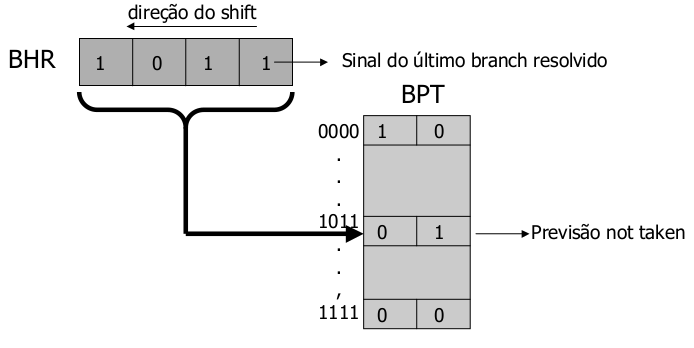
\includegraphics[width=0.85\textwidth]{correlate}
  \caption{Indexação da BHR e BPT na Previsão Correlata}
  \label{fig:correlate}
\end{figure}



\subsubsection{Branch Target Buffer}
Além da previsão da direção, é necessário o endereço da instrução prevista para a execução. Por isso, o \textit{branch target buffer} opera como \textbf{uma cache que guard o endereço previsto da próxima instrução a ser executada após o branch}. Se o PC de uma instrução a ser executada é igual a um PC no BTB, o PC previsto é utilizado como o próximo PC.

Só é necessário guardar os \textit{branches} previstos como \textit{taken}, já que os \textit{branches} não tomados se comportam como as instruções sequenciais.

\begin{figure}[ht]
  \centering
  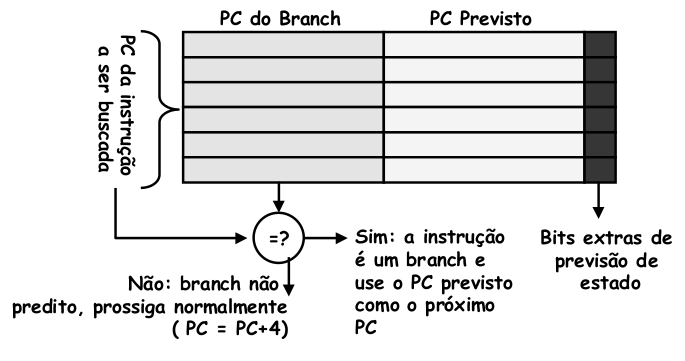
\includegraphics[width=0.85\textwidth]{branch-target-buf}
  \caption{Esquema da previsão dinâmica de buffer, pelo Patterson}
  \label{fig:branch-target-buf}
\end{figure}



\subsection{Execução Especulativa}
A ideia aqui é executar condicionalmente código que está depois de um branch, antes que o branch seja resolvido, o que involve \textbf{a execução do código antes que se tenha certeza de que o mesmo deve ser executado}. É usada em conjunto com a previsão de desvios.

Se a previsão estiver correta, o potencial do ILP é maior do que um caminho do branch. Por isso, o potencial de paralelismo aqui é limitado por duas previsões incorretas (ou \textit{mispredictions}) de direções do branch. A execução especulativa pode ser feita por hardware ou software e temos três tipos, vistos a seguir.



\subsubsection{Single Path}
Neste caso, quando a CPU encontra um branch, o sinal do branch é predito e a
execução prossegue pelo caminho predito. Enquanto o branch não for resolvido, todas as escritas a registradores e memória e todas as operações de I/O devem ser feitas condicionalmente

Estas operações somente serão finalizadas (\textit{committed}) quando todos os branches especulados tiverem sido previstos corretamente. Se houver uma previsão incorreta, as operações não serão finalizas (\textit{squashed}).

O custo em hardware do \textit{single path} é pequeno e cresce linearmente com o número de branches pendentes. Por isso, é o tipo de execução especulativa mais utilizado nos microprocessadores atuais.

\begin{figure}[ht]
  \centering
  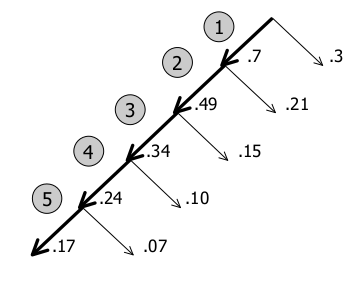
\includegraphics[width=.6\textwidth]{single-path}
  \caption{Exemplo de execução no Simple Path}
  \label{fig:single-path}
\end{figure}




\subsubsection{\textit{Eager Execution}}
Aqui, a execução prossegue pelos dois caminhos do branch, ou seja, não há previsão e sim a execução das duas situações possíveis. Quando um branch é resolvido, todo estado dos caminhos não tomado é descartado.

Sob recursos ilimitados, essa execução oferece o melhor desempenho. Mas com tamanha taxa de descarte e desperdícion, é um algorítmo não realizável.

\begin{figure}[ht]
  \centering
  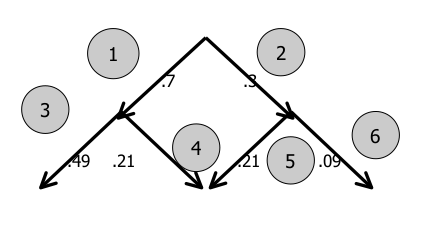
\includegraphics[width=.6\textwidth]{eager-exec}
  \caption{Exemplo de execução no Eager Execution}
  \label{fig:eager-exec}
\end{figure}


\subsubsection{\textit{Disjoint Eager Execution}}
É uma combinação das duas técnicas anteriores, onde os recursos são atribuídos aos branches que tem mais probabilidade de serem executados, considerando todos os branches pendentes. Ou seja, é considerada a probabilidade cumulativa de execução.

Todos os branches são preditos e alguns deles também são executados agressivamente, i. e. os dois caminhos são executados. O custo deste esquema aumenta como uma fração da raiz quadrada do tamanho do caminho principal.

\begin{figure}[ht]
  \centering
  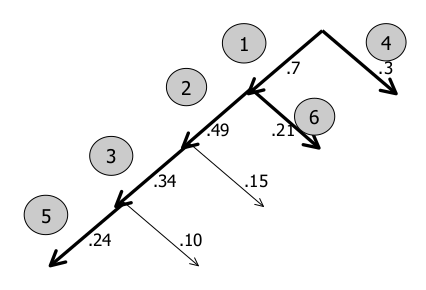
\includegraphics[width=.6\textwidth]{disjoint-eager-exec}
  \caption{Exemplo de execução no Disjoint Eager Execution}
  \label{fig:disjoint-eager-exec}
\end{figure}




\subsection{Arquiteturas Superescalares}
% TODO: indicar se é RISC ou CISC e porque.

\textsc{Definição} Arquiteturas que permitem que diversas instruções sejam iniciadas em um único ciclo de clock e executadas de maneira independente.

Para que isso seja possível, deve-se ser capaz de buscar mais de uma instrução
por ciclo de clock e executar diversas instruções simultaneamente. Entretanto, isso trás uma série de limitações:
\begin{itemize}
  \item \textbf{Dependências}, uma vez que instruções executadas paralelamente podem depender uma da outra;

  \item \textbf{Conflitos estruturais}, onde instruções irão utilizar as mesmas estruturas;

  \item \textbf{Tempos diferentes de execução das instruções}, podendo causar descompassos entre instruções dependentes;

  \item \textbf{Hardware bastante complexo}, dado que a complexidade do hardware depende do número de instruções a serem executadas simultaneamente.
\end{itemize}

\begin{figure}[ht]
  \centering
  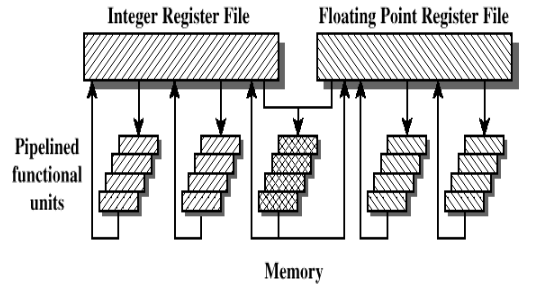
\includegraphics[width=.9\textwidth]{arq-superscalar-org}
  \caption{Organização geral de uma Arquitetura Superescalar}
  \label{fig:arq-superscalar-org}
\end{figure}

\begin{figure}[ht]
  \centering
  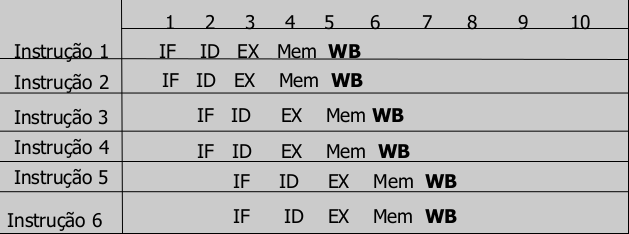
\includegraphics[width=.75\textwidth]{arq-superscalar-exec}
  \caption{Simulação de execução de instruções em Arquitetura Superescalar}
  \label{fig:arq-superscalar-exec}
\end{figure}

O conceito do projeto está muito associado a estruturas RISC, porém pode ser perfeitamente aplicado a estruturas CISC. O Pentium 4 é um exemplo clássico de CISC com arquitetura superescalar. Nele o processador busca as instruções em memória na ordem do programa estático. Porém cada instrução é traduzida em uma ou mais operações RISC de tamanho fixo, chamadas micro-operações. O processador as executa em um pipeline escalar e faz o \textit{commit} de cada uma delas, restaurando o fluxo original do programa. A Figura \ref{fig:pentium4} a arquitetura geral do Pentium 4.

\begin{figure}[ht]
  \centering
  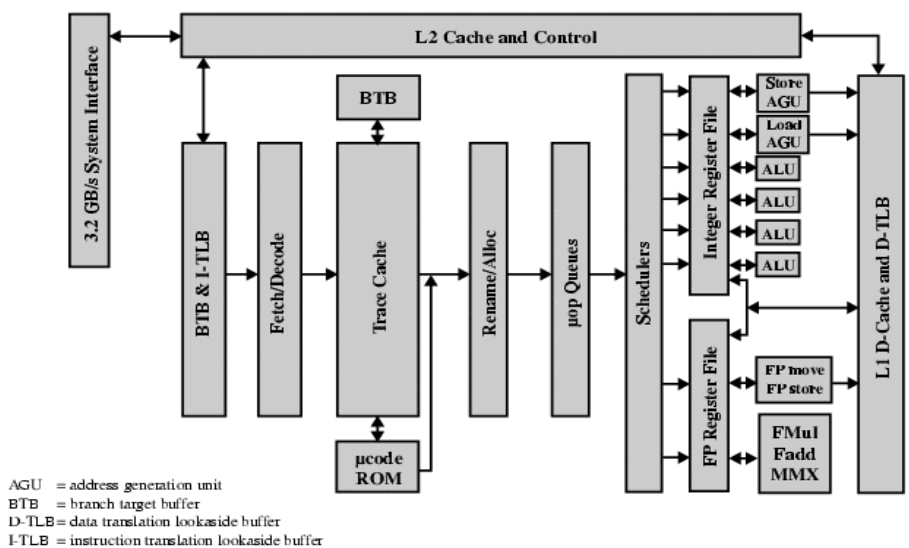
\includegraphics[width=.85\textwidth]{pentium-4}
  \caption{Arquitetura geral do processador do Pentium 4  }
  \label{fig:pentium4}
\end{figure}


\subsection{Very Large Instruction Word - VLIW}
\textsc{Definição} arquitetura que combina diversas operações em uma única instrução muito longa. A tarefa de se determinar quais instruções que serão emitidas simultaneamente, entretanto, recai sobre o compilador.

Neste caso, também teremos diversas unidades funcionais independentes. Uma instrução VLIW poderia incluir 2 operações inteira, 2 de ponto flutuante, 2 referências à memoria e um branch, por exemplo. Dessa forma, se cada unidade funcional tem 16 bits, teríamos um palavra de 112 bits. Note que \textbf{deve haver paralelismo suficiente na sequencia de código para manter todas as unidades ocupadas}.

Como a emissão de instruções e escalonamento é feito pelo compilador, essa arquitetura \textbf{requer pouco ou nenhum \textit{hardware} adicional}. Entretanto, essa abordagem trás alguns problemas:
\begin{itemize}
  \item \textbf{Demandam grande número de portas} sendo uma para cada unidade funcional. Isso aumenta o uso do material - silício - e degrada a velocidade do clock.

  \item Como há múltiplos acessos simultâneos à memória, \textbf{a complexidade da memória também aumenta};

  \item \textbf{O tamanho do código aumenta bastante}, apesar de ser possível a implementação de grande quantidade de \textit{loop unrolling};

  \item Quando as instruções não são totalmente cheias, \textbf{temos espaço disperdiçado na VLIW};

  \item Como as operações são emitidas de maneira síncrona, \textbf{um atraso em qualquer unidade funcional, representa um atraso no processador como um todo}
\end{itemize}

% TODO: indicar se VLIW pode ser conserado RISC ou CISC e porque.
\textbf{Nota:} arquiteturas VLIW não podem ser consideradas RISC ou CISC, mas podem incorporar idéias e implementações destes conjuntos de instruções.



\subsection{Análise de Dependência pelo Compilador}
A análise de dependências é fundamental na exploração do paralelismo, uma vez que a detecção destas em um programa é importante para:
\begin{itemize}
  \item Determinar um bom escalonamento de código

  \item \textbf{Determinar os loops que contém paralelismo}, uma vez que essa propriedade existe quando o \textit{loop} não for \textit{loop-carried}. Note que, entre tanto, \textit{loop-carried} não circulares podem ser eliminadas. As verdadeiras limitantes de paralelismo são as dependências \textit{loop-carried} circulares.

  \item Eliminar dependências de nomes
\end{itemize}

Vemos que a determinação da existência de dependências, no caso geral, é um problema NP-Completo. Porém, existem testes exatos para situações restritas que podem ser aplicados, sendo um \textbf{teste considerado exato quando ele determina precisamente que a dependência existe}.

Além de detectar dependências, o compilador deve ser capaz de classificá-las, permitindo que as dependências de nome sejam resolvidas, já que estão identificadas.

Entretanto, em algumas situações, a análise não é efetiva, principalmente uando existem arrays e ponteiros. Temos os casos:
\begin{itemize}
  \item Objetos referenciados via ponteiros;
  \item Indexação indireta de arrays, através de outro array;
  \item Dependência que existe somente em relação a alguns valores de input.
\end{itemize}
